\documentclass[11pt,a4paper]{article}

\usepackage[margin=1in]{geometry}
\usepackage{graphicx}
\usepackage{amsmath,amssymb,mathtools}
\usepackage{booktabs,array,tabularx,longtable,multirow}
\usepackage{float}
\usepackage{enumitem}
\usepackage{microtype}
\usepackage{hyperref}
\usepackage{tikz}
\usepackage[ruled,vlined,linesnumbered]{algorithm2e}
\usetikzlibrary{arrows.meta,positioning,shapes.geometric,fit,calc}

\hypersetup{colorlinks=true,linkcolor=blue,citecolor=blue,urlcolor=blue}
\setlength{\parskip}{0.35em}
\setlength{\parindent}{1.2em}
\setlist{leftmargin=*,itemsep=0.2em,topsep=0.25em}
\renewcommand{\arraystretch}{1.16}
\newcommand{\method}{\textsc{KryLMC}}
\newcommand{\boa}{\textsc{BOA}}
\newcommand{\lmc}{\textsc{LMC}}
\newcommand{\R}{\mathbb{R}}
\newcommand{\E}{\mathbb{E}}
\newcommand{\D}{\mathcal{D}}
\newcommand{\Krylov}{\mathcal{K}}

\title{\textbf{KryLMC: Progressive Loss Landscape Exploration for Domain Generalization via Krylov Subspace Interpolation}}
\author{Atharva Pratap Singh, Anugrah Singh\\23075013, 23075009}
\date{November 2026}

\begin{document}
\maketitle
\begingroup
\small
\tableofcontents
\endgroup
\newpage

\renewcommand{\abstractname}{1 Abstract}
\begin{abstract}
Deep neural networks can achieve high accuracy on the data distributions used during training and still lose performance when they encounter images collected under unfamiliar conditions. This problem, known as domain generalization, is important in visual recognition systems that must operate across changes in camera hardware, illumination, background, image style, or acquisition environment. A model trained on a limited collection of source domains may rely on visual cues that are correlated with the labels in those domains but are not stable in a new domain. Domain generalization therefore asks whether a model can retain useful predictive behaviour when the target distribution is unavailable during training.

This report studies a post-training approach to this problem through the geometry of the neural network loss landscape. The central observation is that ordinary linear interpolation between two independently fine-tuned networks searches only a one-dimensional path in parameter space. If the path crosses a region of high loss, the best interpolated model may remain close to one of the endpoints and may fail to exploit useful parameter directions outside that segment. The proposed KryLMC framework uses this simple interpolation as a starting point and then performs a structured search in a low-dimensional Krylov subspace. The subspace is built from the gradient of the loss and successive Hessian-vector products at the selected interpolation point. A Billiard-like Optimization Algorithm then moves through the subspace while keeping the training loss within a chosen threshold of the starting loss.

The framework has two stages. First, two models with the same architecture are independently fine-tuned on disjoint halves of a training partition. Their weights are blended at eleven mixing coefficients between zero and one, and the best point is selected as the initial model. Second, a five-dimensional Krylov basis is constructed using finite-difference Hessian-vector products and Gram-Schmidt orthogonalization. BOA performs twenty boundary-reflection steps, producing a trajectory of twenty-one candidate parameter vectors, including the initial point. The reported implementation uses a loss threshold offset of 0.2 for the main experiments and evaluates ResNet-18, ResNet-50, ViT-B/14, ViT-B/16, ViT-B/32, and Mamba.

The supplied manuscript reports results on PACS, VLCS, TerraIncognita, and OfficeHome. In the direct comparison table, Krylov refinement improves all six architectures on VLCS by between 0.5 and 2.5 percentage points and all six architectures on TerraIncognita by approximately 2.2 to 2.3 points. On PACS, the four architectures for which a direct naive-versus-Krylov comparison is reported show no improvement. OfficeHome accuracies are listed, but corresponding naive interpolation results are not supplied. DomainNet is described as a benchmark but no numerical result is reported for it. The ablation studies examine random subspaces, gradient-only directions, and Krylov dimension on ResNet-18/PACS with Sketch held out; they provide geometric diagnostics, but the accuracy improvements are not consistent across random seeds.

The evidence therefore supports a measured conclusion: curvature-informed post-training exploration can improve the reported interpolation baseline in the evaluated VLCS and TerraIncognita settings, but the current results do not establish a general improvement for every dataset or a fully controlled unseen-domain claim. The report records the experimental protocol and its limitations explicitly, including the use of a pooled random train-test split in the main evaluation and the selection of candidate models on the same held-out split used for reporting accuracy. Further experiments with domain-wise holdouts, independent validation and test sets, repeated seeds, and completed DomainNet evaluation are needed before stronger claims can be made.
\end{abstract}
\addcontentsline{toc}{section}{\protect\numberline{1}Abstract}
\setcounter{section}{1}

\section{Introduction}

\subsection{Motivation and context}
Deep learning has become a standard approach to image classification because a sufficiently expressive model can learn useful visual representations from large collections of labelled images. In many practical settings, however, the data available during development do not cover every condition that will occur after deployment. Images may be captured by different cameras, under different lighting, against new backgrounds, or with different visual styles. These changes can alter the distribution of input features even when the object categories remain the same. A classifier that performs well on one collection may consequently make more errors on another collection drawn from a different environment.

This setting is commonly described through distribution shift. Let a source domain be represented by a joint distribution $P_S(x,y)$ over an image $x$ and its label $y$. At deployment, the model may encounter a target distribution $P_T(x,y)$ that differs from the source distribution. Domain adaptation attempts to use some information from the target domain during training or adaptation. Domain generalization addresses the more restrictive case in which the target domain is not available during training. Instead, the learner receives data from one or more source domains and must learn a predictor that remains useful on a previously unseen target domain \cite{quinonero2009dataset,bendavid2010theory,blanchard2011generalizing,muandet2013domain}.

The problem is not limited to a particular network architecture. Convolutional networks, vision transformers, and newer state-space models can all learn features that perform well on the observed training distribution. Their performance under a new distribution depends on whether the learned representation captures stable information about the label or relies on incidental properties of the source data. A model may, for example, associate an object with a background, a texture, or a camera-specific pattern that happens to be predictive in the training set. Such correlations may weaken or disappear in another environment.

A widely used starting point is empirical risk minimization (ERM), which minimizes the average loss over the available training samples. ERM is simple and often competitive, but it does not directly constrain how the model behaves when the input distribution changes. A broad empirical study of domain generalization methods found that carefully tuned ERM remains a strong baseline and that specialised methods do not improve consistently across settings \cite{gulrajani2021search}. This makes it important to examine methods that can improve robustness without adding substantial complexity to the original training procedure.

\subsection{Why examine the loss landscape?}
Training a neural network can be viewed as searching for parameters that minimize a loss function $\mathcal{L}(\theta)$, where $\theta\in\R^d$ contains all trainable parameters. The loss landscape describes how the objective changes as the parameters move. A narrow basin in which small parameter changes cause a rapid increase in loss is often called sharp. A wider region in which the loss changes more gradually is commonly called flat. Earlier studies have connected flat minima with generalization, although subsequent work has shown that sharpness is sensitive to parameterization and is not, by itself, a universal guarantee of generalization \cite{hochreiter1997flat,keskar2017large,dinh2017sharp,jiang2020fantastic}.

A common way to express local sensitivity is the worst-case increase in loss inside a neighbourhood of radius $\rho$:
\begin{equation}
 s_{\rho}(\theta)=\max_{\|\epsilon\|_2\leq\rho}
 \left[\mathcal{L}(\theta+\epsilon)-\mathcal{L}(\theta)\right].
 \label{eq:sharpness}
\end{equation}
A smaller value indicates that the loss is less sensitive to perturbations within that neighbourhood. Flatness is therefore a useful geometric quantity to study, but it should be treated as a motivation and an empirical signal rather than as a mathematical guarantee of out-of-domain accuracy.

Several training-time methods explicitly seek flatter solutions. Sharpness-Aware Minimization (SAM), for example, uses a local perturbation to estimate a direction of high loss and updates the model using the perturbed objective \cite{foret2021sharpness}. Domain-generalization methods such as SWAD and sharpness-aware gradient matching adapt this general idea to improve performance across domains \cite{cha2021swad,wang2023sagm}. These approaches modify the training objective or optimization procedure. Their additional training cost can be meaningful when the original models are already trained or when retraining is undesirable.

\subsection{Interpolation as a post-training alternative}
Linear mode connectivity studies whether two neural networks can be joined by a low-loss path in parameter space. Given two parameter vectors $\theta_1$ and $\theta_2$, linear interpolation defines
\begin{equation}
 \theta(\alpha)=\alpha\theta_1+(1-\alpha)\theta_2,
 \qquad 0\leq\alpha\leq1.
 \label{eq:linear_interpolation}
\end{equation}
If the two solutions lie in a compatible region of the loss landscape, some intermediate points can perform as well as or better than either endpoint. Linear mode connectivity and model averaging have been studied in neural network optimization, model ensembling, and model merging \cite{garipov2018loss,draxler2018barriers,frankle2020linear,izmailov2018swa,wortsman2022soups}.

The limitation of the simple interpolation path is geometric. It explores only the line segment between the two endpoints. If the loss rises sharply around the middle of that segment, the search cannot move around the barrier. The best point on the line may then be close to one of the original models. A richer search would need directions that reflect the local geometry of the loss surface rather than directions chosen only by the two endpoints.

\subsection{Research direction}
Krylov subspaces offer a way to construct a compact set of directions from matrix-vector products. In this work, the matrix is the Hessian of the loss at the best point obtained from naive interpolation, and the initial vector is the gradient at that point. The resulting basis contains first-order information and directions shaped by successive applications of local curvature. The Hessian itself is not formed explicitly; Hessian-vector products can be computed through gradient evaluations or equivalent automatic-differentiation procedures \cite{pearlmutter1994hessian,liesen2013krylov,vinyals2012krylov}.

The report studies a progressive interpolation strategy called KryLMC. A naive interpolation stage first provides a reasonable starting point. A Krylov subspace and a Billiard-like Optimization Algorithm then explore a bounded region around it. The intention is to retain the computational convenience of post-training model interpolation while allowing the search to leave the original straight line. The method is evaluated on six architectures and four datasets with reported accuracy tables. The remainder of this report describes the relevant literature, formal problem, method, implementation, results, ablations, limitations, and a concrete application scenario.

\section{Related Work}

\subsection{Domain generalization and invariant representations}
Domain generalization has been studied through several complementary perspectives. Early theoretical formulations considered how a learner can construct predictors that transfer across environments when the target distribution is not observed \cite{blanchard2011generalizing,muandet2013domain,bendavid2010theory}. One family of methods attempts to remove domain-specific information from the learned representation. Domain-adversarial neural networks train a feature extractor together with a domain classifier and encourage the feature extractor to make source domains difficult to distinguish \cite{ganin2016dann}. Conditional invariant representation learning and related approaches seek to preserve label-relevant information while reducing domain dependence \cite{li2018conditional,arjovsky2019irm}.

The appeal of invariant representation learning is clear: features that capture stable object properties may transfer better than features tied to a particular environment. However, domain invariance is not automatically equivalent to predictive usefulness. A domain discriminator can suppress information that is both domain-related and label-relevant. Adversarial objectives may also be sensitive to optimization settings and the relative strength of the competing losses. The supplied paper therefore treats invariant feature learning as an important line of prior work, but takes a different route by operating on model parameters after training rather than adding a domain discriminator to the training objective.

\subsection{Meta-learning and episodic training}
Meta-learning methods construct training episodes that simulate a sequence of source and target environments. Model-Agnostic Meta-Learning learns an initialization that can adapt quickly through a small number of gradient updates \cite{finn2017maml}. Domain-generalization variants use source-domain partitions to encourage a model to learn update behaviour that transfers to held-out environments. MetaReg, for example, uses meta-regularization to improve transfer across domains \cite{balaji2018metareg}. Learning-to-generalize formulations similarly use episodic domain splits to expose the learner to simulated distribution changes \cite{li2018learninggeneralize}.

These methods provide a direct way to train for domain shift, but they require careful episode construction and additional optimization. Their results can depend on whether the simulated training shifts resemble the actual deployment shift. KryLMC is complementary: it does not introduce an episodic training objective and instead refines already-trained weights. It should not be interpreted as a substitute for meta-learning in every setting, because the two approaches address different points in the training pipeline.

\subsection{Data augmentation and synthetic domain variation}
Data augmentation attempts to make the training distribution more diverse. MixStyle perturbs feature statistics to simulate changes in appearance \cite{zhou2021mixstyle}. Random convolution methods create alternative image appearances without requiring a separately trained style-transfer model \cite{xu2021randomconv}. Fourier-based methods modify frequency components to change image style while retaining much of the underlying semantic structure \cite{xu2021fourier}. Generative and adversarial augmentation methods have also been used to produce challenging training examples \cite{volpi2018adversarial,zhou2020deep}.

Augmentation can be simple to combine with standard training, but its value depends on the range of transformations used. When the true deployment shift is unknown, no fixed collection of transformations can guarantee that all relevant changes have been represented. KryLMC does not add synthetic samples. It changes the selected parameter vector after the two source models have been trained, so the method can in principle be combined with an augmentation-based training pipeline.

\subsection{Flat minima and sharpness-aware optimization}
The relation between loss geometry and generalization has motivated studies of sharp and flat minima, visualization of neural loss surfaces, and measures of generalization based on local curvature \cite{li2018visualizing,hochreiter1997flat,keskar2017large,jiang2020fantastic}. Sharpness-Aware Minimization explicitly seeks parameter updates that perform well in a neighbourhood around the current model \cite{foret2021sharpness}. SWAD applies a flat-minimum perspective to domain generalization by averaging weights over a suitable training trajectory \cite{cha2021swad}. More recent sharpness-aware domain-generalization approaches refine the objective or gradients to improve robustness under shifts \cite{wang2023sagm,li2025consistent,song2025dgsam}.

These methods provide evidence that the neighbourhood around a solution can matter, but they typically change the training process. KryLMC instead treats the output of existing training as input to a separate interpolation procedure. The distinction is practical: KryLMC avoids retraining the full model during the interpolation stage, although it still incurs gradient and Hessian-vector-product computation when constructing the Krylov basis and evaluating the BOA trajectory.

The connection between flatness and generalization must also be interpreted carefully. Sharp minima can generalize well under certain parameter transformations, and different sharpness measures can produce different rankings of models \cite{dinh2017sharp,wen2023sharpness,zhang2021flatness}. Accordingly, the present work does not establish a theorem that flatter models always achieve better target-domain accuracy. Its claim is empirical: a curvature-informed search can identify useful parameter vectors in some of the evaluated cases.

\subsection{Linear mode connectivity and model merging}
Linear mode connectivity describes low-loss paths between independently trained neural networks. Studies have examined the topology of neural loss surfaces and shown that apparently separate solutions can sometimes be connected by curves or paths with low loss \cite{garipov2018loss,draxler2018barriers,frankle2020linear}. Weight averaging, including Stochastic Weight Averaging and model soups, has shown that combining compatible parameter vectors can improve or preserve predictive accuracy without increasing inference cost \cite{izmailov2018swa,wortsman2022soups}. Model merging and permutation alignment methods further examine how independently fine-tuned networks can be combined \cite{ainsworth2023git,entezari2022permutation,ilharco2023taskarithmetic}.

The naive version of LMC uses a scalar interpolation coefficient and therefore examines a single straight segment. This is computationally attractive, but its search space is narrow. KryLMC uses the best naive interpolation point as an anchor and adds a structured local subspace. The interpolation stage and the Krylov stage consequently have different roles: one combines the two endpoints, while the other explores directions derived from the local loss geometry.

\subsection{Krylov methods and Hessian-vector products}
Krylov subspaces are standard tools in numerical linear algebra. Given a matrix $H$ and a nonzero vector $g$, a Krylov subspace of order $K$ is
\begin{equation}
 \Krylov_K(H,g)=\operatorname{span}\{g,Hg,H^2g,\ldots,H^{K-1}g\}.
 \label{eq:krylov_general}
\end{equation}
Such spaces are used in iterative methods for large linear systems and eigenvalue problems because they can capture useful information without explicitly computing a complete matrix decomposition \cite{saad2003iterative,liesen2013krylov}. In neural networks, Hessian-vector products provide a way to access second-order information without storing the full Hessian, whose dimension grows quadratically with the number of parameters \cite{pearlmutter1994hessian,martens2010hessianfree}.

Prior work has explored Krylov subspace methods for deep learning optimization and domain generalization. The supplied manuscript cites the 2026 work on mode connectivity in Krylov subspaces as the source of the BOA-based search mechanism \cite{li2026krylovboa}. The present report should therefore position its contribution carefully: the Billiard-like search and the use of Krylov directions are not claimed as wholly new mathematical inventions. The work under study combines a naive LMC warm start with this curvature-informed search and evaluates the resulting progressive procedure across several architecture families.

\subsection{Position of the present work}
KryLMC lies at the intersection of domain generalization, post-training model interpolation, and local loss-landscape exploration. It differs from methods that improve domain generalization only by changing the training objective, because it begins from two already fine-tuned models. It differs from naive model averaging because it can move away from the line between the two weight vectors. Its central design choice is to restrict that additional search to a low-dimensional subspace constructed from gradient and curvature information. This makes the method more structured than an arbitrary random search, but it also introduces extra gradient computations and requires care when interpreting candidate selection and evaluation results.

\section{Research Gap}

The supplied literature and experiments point to a specific gap between two common approaches. Training-time methods can explicitly encourage domain-invariant representations or flatter solutions, but they require changes to model training. Post-training interpolation is easier to apply to existing models, but ordinary linear interpolation is restricted to a single path. When that path crosses a high-loss region, a scalar interpolation coefficient cannot move around the barrier, even if a better region exists in a nearby direction.

The gap is therefore not simply the absence of another domain-generalization loss. It is the limited geometry of the post-training search. A method that begins from independently trained models and then explores additional directions should ideally satisfy three properties. First, its search space should be substantially smaller than the full parameter space, since contemporary networks contain millions of parameters. Second, the directions should be related to the loss landscape rather than chosen without regard to the local objective. Third, the procedure should keep candidate parameters within a controlled loss region so that exploration does not move arbitrarily far from the starting solution.

Krylov subspaces are a natural candidate for constructing such directions. The initial gradient contributes first-order information, while Hessian-vector products add curvature information. BOA then uses the projected gradient at a boundary point to reflect the current search direction. This offers a mechanism for exploring a bounded region using a small number of directions. The method is post-training in the sense that it does not update the original training objective or repeat the full fine-tuning process. It is not computation-free, because basis construction, line searches, and candidate evaluations still require substantial work.

\subsection{Motivating evidence in the supplied experiments}
The reported interpolation analysis provides an example of why a one-dimensional path can be restrictive. On TerraIncognita, the ResNet-18 interpolation curve is reported to fall from 54.5\% at one endpoint to approximately 47.8\% near the midpoint. The best Krylov-refined result is 56.7\%, a reported gain of 2.2 percentage points over the naive LMC value of 54.5\%. The corresponding results for all six architectures show improvements between 2.2 and 2.3 points. These observations motivate a search that can leave the line segment when an interpolation barrier is present.

On VLCS, the reported gains are smaller but positive for all six architectures, ranging from 0.5 to 2.5 percentage points. On PACS, four architectures in the direct comparison table show no improvement over naive LMC. This contrast suggests that the benefit of the second stage depends on the starting geometry: when naive interpolation already produces a strong candidate, the available improvement may be small; when the interpolation path exhibits a barrier, the additional search may be more useful.

\begin{table}[H]
\centering
\caption{Motivating comparison reported in the supplied manuscript. Values are test accuracy percentages.}
\label{tab:motivation}
\begin{tabular}{lccc}
\toprule
Setting & Naive LMC & Krylov LMC & Difference \\
\midrule
TerraIncognita, ResNet-18 & 54.5 & 56.7 & +2.2 \\
VLCS, ViT-B/16 & 82.0 & 84.5 & +2.5 \\
PACS, ViT-B/16 & 98.6 & 98.6 & 0.0 \\
\bottomrule
\end{tabular}
\end{table}

\subsection{Protocol gap that remains unresolved}
A central limitation must be stated alongside the motivation. In the main experimental protocol, the domains of each dataset are pooled and then randomly divided into an 80\% training portion and a 20\% held-out portion. This leaves images from the same named domains represented in both portions. Such a split measures generalization to held-out images from a mixture of observed domains; it is not equivalent to the strict domain-generalization protocol in which an entire domain is excluded from training. The ablation section separately describes PACS with Sketch held out as the unseen domain. These are different evaluation settings and should not be conflated.

There is a second issue: the same held-out split is used to select the best interpolation coefficient and the best BOA candidate, and then to report the chosen candidate's accuracy. This can bias the reported estimate upward because the evaluation set participates in model selection. A clean evaluation should use a validation split for choosing $\alpha$ and the BOA candidate and a separate untouched test split for final reporting. The current report records the protocol as described in the source and treats the results as evidence requiring further validation, not as a definitive demonstration of unseen-domain generalization.

\section{Problem Statement}

Let $\mathcal{X}$ denote the image space and $\mathcal{Y}$ the set of class labels. Suppose the available data are collected from $M$ source domains with distributions $P_1,\ldots,P_M$. The target domain has an unknown distribution $P_T$ and is unavailable during the training stage. A predictor $f_\theta:\mathcal{X}\rightarrow\mathcal{Y}$ is parameterized by $\theta\in\R^d$. The domain-generalization objective is to obtain parameters that achieve low expected target risk
\begin{equation}
 R_T(\theta)=\E_{(x,y)\sim P_T}\left[\ell(f_\theta(x),y)\right],
 \label{eq:target_risk}
\end{equation}
using only information available from the source domains. Since $P_T$ is unknown, the target risk cannot be optimized directly during training.

The method considered here starts from two parameter vectors $\theta_1$ and $\theta_2$ obtained by independently fine-tuning models of the same architecture. Naive linear mode connectivity searches the segment
\begin{equation}
 \Theta_{\mathrm{line}}=\left\{\alpha\theta_1+(1-\alpha)\theta_2:0\leq\alpha\leq1\right\}.
 \label{eq:line_set}
\end{equation}
For a chosen empirical loss $\mathcal{L}$, the best point on this discretized segment is used as the anchor
\begin{equation}
 \theta_0=\theta(\alpha^*),\qquad
 \alpha^*\in\{0,0.1,0.2,\ldots,1.0\}.
 \label{eq:anchor}
\end{equation}
The central limitation is that $\Theta_{\mathrm{line}}$ contains only one degree of freedom. If the best region is not located on this segment, naive interpolation cannot reach it.

KryLMC expands the search to a low-dimensional affine subspace around $\theta_0$. Let $H_0=\nabla^2_\theta\mathcal{L}(\theta_0)$ and $g_0=\nabla_\theta\mathcal{L}(\theta_0)$. A $K$-dimensional basis is constructed from
\begin{equation}
 \Krylov_K(H_0,g_0)=\operatorname{span}\{g_0,H_0g_0,\ldots,H_0^{K-1}g_0\}.
 \label{eq:problem_krylov}
\end{equation}
Let $V=[v_1,\ldots,v_K]\in\R^{d\times K}$ contain orthonormal basis vectors. The explored parameter set is
\begin{equation}
 \Theta_{\mathrm{sub}}=\{\theta_0+Vc:c\in\R^K\}.
 \label{eq:affine_subspace}
\end{equation}

The search is constrained by a loss threshold
\begin{equation}
 \mathcal{L}(\theta)\leq\mathcal{L}(\theta_0)+\delta,
 \label{eq:loss_constraint}
\end{equation}
where $\delta$ is a non-negative tolerance. Within this constrained region, BOA generates a trajectory of candidates by alternating boundary search and reflection. The practical selection objective in the supplied implementation is top-1 accuracy on the held-out evaluation split. Because that same split is also used to report the final accuracy, the reported selection procedure is not an independent estimate of test performance.

The resulting problem can be summarized as follows: given two independently trained models of the same architecture, construct a low-dimensional, curvature-aware neighbourhood around their best naive interpolation point and search within a loss-bounded region for a parameter vector that improves empirical classification performance. The research question is whether the additional directions provided by the Krylov basis allow BOA to find better candidates than the one-dimensional interpolation path, and under what data and architecture conditions such improvements are observed.

This is an empirical optimization problem, not a theorem asserting that a flat minimum must minimize target risk. The mathematical formulation defines the search space and constraint. Experimental validation is needed to determine whether the candidates selected by this procedure actually generalize to new domains.

\section{Novel Contribution}

The contributions supported by the supplied work are best understood as a progressive framework and an empirical study, rather than as the invention of every component used by the method.

\begin{enumerate}
 \item \textbf{A two-stage post-training pipeline.} The method uses naive linear interpolation as an inexpensive warm start and then refines the selected point through a curvature-informed subspace. This separates the simple model-combination step from the more expensive geometric exploration step.
 \item \textbf{Krylov directions for local parameter exploration.} The basis is seeded by the gradient at the naive interpolation point and extended through Hessian-vector products. Compared with a random basis, this construction supplies directions tied to the local objective. The source experiments show a theoretical alignment of $1/\sqrt{K}$ between the initial direction and the negative gradient under the stated orthonormal-basis construction.
 \item \textbf{Loss-bounded trajectory exploration.} BOA uses a fixed loss threshold and boundary reflections to generate candidate parameters inside a controlled region. This gives the search a geometric stopping boundary rather than allowing unrestricted movement in parameter space.
 \item \textbf{Evaluation across distinct architecture families.} The supplied manuscript reports results for ResNet-18, ResNet-50, three Vision Transformer variants, and Mamba. This permits an initial comparison of the method across convolutional, attention-based, and state-space model families.
 \item \textbf{Diagnostic ablations.} The work compares Krylov directions with random and gradient-only subspaces and studies different Krylov dimensions. These studies investigate whether the curvature information changes the behaviour of BOA, even when the measured accuracy difference is small or unstable across seeds.
\end{enumerate}

The main design motivation is the limitation of a one-dimensional interpolation path. A random subspace adds directions but offers no systematic relationship to the local loss. A gradient-only subspace uses first-order information but does not explicitly encode how the loss curves away from the anchor. Krylov construction is selected because repeated Hessian-vector products add local curvature information while retaining a small basis dimension. The experiments suggest that this geometric structure can make the BOA boundary search more meaningful. They do not, however, establish that $K=5$ is optimal for all architectures or datasets, nor that the method consistently improves accuracy in every setting.

\section{Complete Proposed Methodology}

\subsection{Framework overview}
KryLMC operates after two models of the same architecture have been fine-tuned. It has two sequential stages: naive LMC interpolation and Krylov-subspace exploration with BOA. The first stage combines model parameters along a line. The second uses a compact subspace around the selected interpolation point and searches within a loss-bounded region.

\begin{figure}[H]
\centering
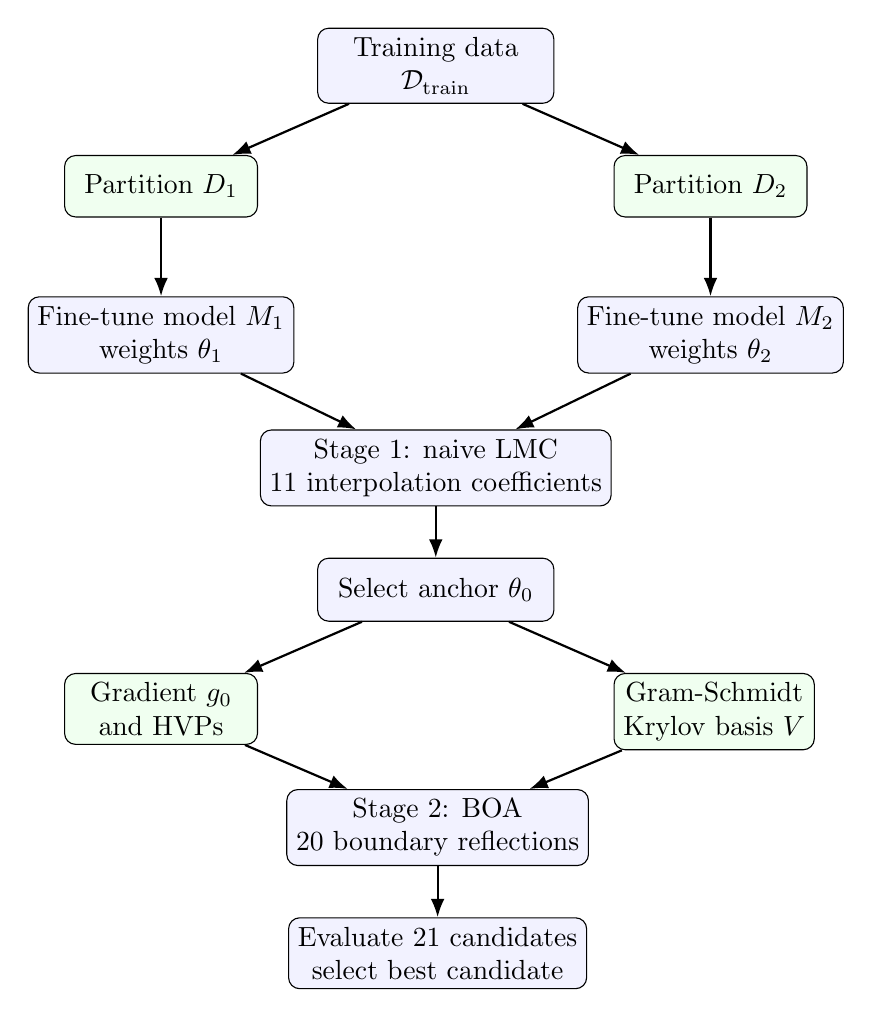
\begin{tikzpicture}[
 node distance=0.65cm and 0.55cm,
 block/.style={draw,rounded corners,align=center,minimum width=3.0cm,minimum height=0.8cm,fill=blue!5},
 smallblock/.style={draw,rounded corners,align=center,minimum width=2.45cm,minimum height=0.78cm,fill=green!6},
 line/.style={-Latex,thick}
]
\node[block] (data) {Training data\\$\mathcal{D}_{\mathrm{train}}$};
\node[smallblock,below left=of data,xshift=-0.2cm] (d1) {Partition $D_1$};
\node[smallblock,below right=of data,xshift=0.2cm] (d2) {Partition $D_2$};
\node[block,below=1.0cm of d1] (m1) {Fine-tune model $M_1$\\weights $\theta_1$};
\node[block,below=1.0cm of d2] (m2) {Fine-tune model $M_2$\\weights $\theta_2$};
\node[block,below=1.2cm of $(m1)!0.5!(m2)$] (lmc) {Stage 1: naive LMC\\11 interpolation coefficients};
\node[block,below=of lmc] (anchor) {Select anchor $\theta_0$};
\node[smallblock,below left=of anchor,xshift=-0.2cm] (grad) {Gradient $g_0$\\and HVPs};
\node[smallblock,below right=of anchor,xshift=0.2cm] (basis) {Gram-Schmidt\\Krylov basis $V$};
\node[block,below=1.0cm of $(grad)!0.5!(basis)$] (boa) {Stage 2: BOA\\20 boundary reflections};
\node[block,below=of boa] (select) {Evaluate 21 candidates\\select best candidate};
\draw[line] (data) -- (d1);
\draw[line] (data) -- (d2);
\draw[line] (d1) -- (m1);
\draw[line] (d2) -- (m2);
\draw[line] (m1) -- (lmc);
\draw[line] (m2) -- (lmc);
\draw[line] (lmc) -- (anchor);
\draw[line] (anchor) -- (grad);
\draw[line] (anchor) -- (basis);
\draw[line] (grad) -- (boa);
\draw[line] (basis) -- (boa);
\draw[line] (boa) -- (select);
\end{tikzpicture}
\caption{Overview of the two-stage KryLMC workflow. The diagram summarizes the pipeline described in the supplied manuscript.}
\label{fig:kry_lmc_framework}
\end{figure}

\subsection{Data partitioning and independent model training}
Let $\mathcal{D}$ denote the image dataset used in an experiment. The supplied implementation first divides the pooled dataset into an 80\% training split and a 20\% held-out split using random seed 42. The training portion is then divided into two equal, disjoint subsets $D_1$ and $D_2$. Two models, $M_1$ and $M_2$, with identical architectures are initialized from the specified pretrained weights and fine-tuned independently on these subsets.

The partitioning is intended to produce two different parameter vectors while retaining the same architecture and output-label space. If the two models are trained on exactly the same samples with identical optimization settings, their weights may be less diverse, reducing the potential value of interpolation. Training on disjoint subsets creates different training histories and offers two parameter vectors that can be combined.

The source specifies ImageNet-pretrained initialization for the model families, with DINOv2 weights for ViT-B/14 and ImageNet-21K weights for ViT-B/16 and ViT-B/32. The exact training schedule is architecture-dependent and is listed in the Implementation Details section. The supplied manuscript does not provide a hardware model, GPU memory size, or a full per-dataset training-time breakdown; those details should be added from the experiment logs before final submission.

\subsection{Stage 1: naive linear mode connectivity}
After fine-tuning, the parameter vectors of the two models are denoted by $\theta_1$ and $\theta_2$. The interpolation stage constructs
\begin{equation}
 \theta(\alpha)=\alpha\theta_1+(1-\alpha)\theta_2,
 \quad \alpha\in\{0.0,0.1,\ldots,1.0\}.
 \label{eq:stage1}
\end{equation}
Each of the eleven candidate models is evaluated, and the best coefficient is denoted by $\alpha^*$. The corresponding weights form the anchor point $\theta_0=\theta(\alpha^*)$. This stage requires no additional gradient-based retraining. It is a direct parameter interpolation followed by model evaluation.

The method assumes that the corresponding parameters of the two networks are aligned sufficiently well for direct interpolation to be meaningful. This is a non-trivial assumption for independently trained neural networks because hidden units and channels can be permuted without changing the represented function. The supplied work uses identical architectures and pretrained initialization, but it does not describe an explicit permutation-matching step. The limitation should be kept in mind when interpreting the interpolation curves.

\subsection{Stage 2: Krylov subspace construction}
The second stage starts from $\theta_0$. It uses the gradient
\begin{equation}
 g_0=\nabla_\theta\mathcal{L}(\theta_0)
 \label{eq:g0}
\end{equation}
computed using a fixed set of training batches. The gradient is normalized and used as the initial Krylov direction. Let $H_0=\nabla^2_\theta\mathcal{L}(\theta_0)$ denote the Hessian at the anchor. The desired basis spans
\begin{equation}
 \Krylov_K(H_0,g_0)=\operatorname{span}
 \{g_0,H_0g_0,H_0^2g_0,\ldots,H_0^{K-1}g_0\}.
 \label{eq:krylov_basis}
\end{equation}
The main configuration uses $K=5$.

The full Hessian is not explicitly formed. The supplied manuscript describes a finite-difference approximation to the Hessian-vector product:
\begin{equation}
 H_0v\approx\frac{\nabla\mathcal{L}(\theta_0+\varepsilon v)
 -\nabla\mathcal{L}(\theta_0)}{\varepsilon},
 \qquad \varepsilon=10^{-3}.
 \label{eq:finite_difference_hvp}
\end{equation}
This approximation estimates how the gradient changes along the vector $v$. It avoids storing a dense $d\times d$ Hessian, which would be impractical for a model with millions of parameters.

Starting from the normalized gradient, the method repeatedly applies the Hessian-vector operator and orthogonalizes each new vector against the previous basis vectors using Gram-Schmidt. If $w_k$ is the vector produced by the next Hessian-vector product, its orthogonal component is
\begin{equation}
 \widetilde{v}_k=w_k-\sum_{j=1}^{k-1}
 \langle w_k,v_j\rangle v_j,
 \qquad
 v_k=\frac{\widetilde{v}_k}{\|\widetilde{v}_k\|_2}.
 \label{eq:gram_schmidt}
\end{equation}
The procedure yields the orthonormal basis $V=[v_1,\ldots,v_K]$. If a residual norm becomes numerically negligible, a practical implementation should detect rank loss rather than divide by a near-zero value. The supplied paper studies this issue in the dimensionality ablation, where later Krylov vectors contribute progressively less new information.

\subsection{Stage 2: Billiard-like Optimization Algorithm}
After constructing the basis, BOA explores parameter vectors of the form $\theta_0+Vc$. The starting direction is defined as
\begin{equation}
 p_0=-\frac{\sum_{k=1}^{K}v_k}
 {\left\|\sum_{k=1}^{K}v_k\right\|_2}.
 \label{eq:p0}
\end{equation}
Since the first basis vector is the normalized gradient and the basis is orthonormal, the initial direction has a predictable component along the negative gradient. For the construction used in the ablations, this alignment is $1/\sqrt{K}$.

The allowed region is defined using the loss at the anchor:
\begin{equation}
 \mathcal{L}_{\mathrm{limit}}=\mathcal{L}(\theta_0)+\delta,
 \qquad \delta=0.2
 \label{eq:loss_limit}
\end{equation}
for the main pipeline. Starting from $\theta_i$, the algorithm searches along $p_i$ for a step length $\beta_i$ that reaches the loss boundary:
\begin{equation}
 \theta_{i+1}=\theta_i+\beta_i p_i,
 \qquad
 \mathcal{L}(\theta_{i+1})\approx\mathcal{L}_{\mathrm{limit}}.
 \label{eq:boa_step}
\end{equation}
The line search described in the source uses an expansion phase to bracket the boundary, refinement by bisection, and a golden-section search to locate the crossing. The maximum step size is 5.0 in the main configuration.

At the boundary, the gradient is projected into the Krylov subspace and normalized to obtain a local normal direction $n_i$. The incoming direction is reflected according to
\begin{equation}
 p_{i+1}=p_i-2(p_i^Tn_i)n_i.
 \label{eq:boa_reflection}
\end{equation}
This operation changes the direction of travel while keeping the search associated with the same loss-bounded region. Twenty reflection steps are performed. Together with the starting point, this yields twenty-one candidate parameter vectors.

The source evaluates each trajectory point on the held-out split and retains the candidate with the highest top-1 accuracy. This is the reported model-selection rule. As noted earlier, using the same split for selection and final reporting is a methodological limitation. A revised experiment should choose the best candidate on a validation partition and report its performance once on an independent test partition.

\subsection{Model architectures}
The experiments cover six model families or variants:
\begin{itemize}
 \item ResNet-18 and ResNet-50 are convolutional neural networks with residual connections. The manuscript reports approximately 11 million parameters for ResNet-18 and approximately 25 million for ResNet-50.
 \item ViT-B/14, ViT-B/16, and ViT-B/32 are Vision Transformer variants. The reported models use 12 attention heads and 768-dimensional embeddings. Their patch sizes and input resolutions differ.
 \item Mamba is a state-space architecture included to test the framework beyond convolutional and attention-based models.
\end{itemize}
ResNet models use ImageNet-1K initialization. ViT-B/14 uses DINOv2 pretrained weights, while ViT-B/16 and ViT-B/32 use ImageNet-21K initialization. The source describes Mamba as using ImageNet-1K initialization. The exact Mamba model variant and checkpoint identifier should be added from the implementation configuration before final submission.

\subsection{End-to-end data flow}
The complete workflow can be summarized as follows. The pooled training data are divided into two disjoint subsets. Two models of the same architecture are trained separately. Their weights are interpolated at eleven coefficients. The best interpolation point becomes the anchor. The gradient and Hessian-vector products at that anchor define a five-dimensional Krylov basis. BOA then produces twenty reflected boundary points, and the final candidate is selected from the twenty-one available points. The selected parameter vector is then used for inference.

\section{Overall Optimization}

\subsection{Training objective}
For a source training set $\D_{\mathrm{train}}=\{(x_i,y_i)\}_{i=1}^{N}$, the empirical classification objective can be written as
\begin{equation}
 \mathcal{L}(\theta)=\frac{1}{N}\sum_{i=1}^{N}
 \ell(f_\theta(x_i),y_i),
 \label{eq:empirical_loss}
\end{equation}
where $\ell$ is the classification loss used by the implementation. The supplied manuscript does not explicitly state the loss function by name in the portions provided; cross-entropy is common for this task, but it should not be inserted as a confirmed implementation detail until the code or experiment configuration is checked. In the present report, $\mathcal{L}$ is therefore left as the empirical training loss used by the source implementation.

The two models are trained on $D_1$ and $D_2$ respectively. Each training run minimizes its empirical objective using Adam. The optimization schedules differ by architecture family. The objective of this training stage is not to solve the target-domain optimization problem directly, since the target distribution is unavailable. Rather, it produces two parameter vectors whose interpolation can be studied.

\subsection{Naive interpolation search}
The first optimization stage is a finite search over eleven parameter combinations. Define
\begin{equation}
 \mathcal{A}=\{0,0.1,0.2,\ldots,1.0\}.
\end{equation}
For each $\alpha\in\mathcal{A}$, construct $\theta(\alpha)$ using Equation~\eqref{eq:stage1}. The best coefficient is
\begin{equation}
 \alpha^*=\arg\max_{\alpha\in\mathcal{A}}
 \operatorname{Acc}_{\mathrm{eval}}(\theta(\alpha)),
 \qquad \theta_0=\theta(\alpha^*).
 \label{eq:alpha_star}
\end{equation}
The evaluation metric in the supplied manuscript is top-1 accuracy. The equation describes the reported selection rule; for an unbiased final evaluation, $\operatorname{Acc}_{\mathrm{eval}}$ should be replaced during selection by validation accuracy and the final test set should remain untouched.

\subsection{Krylov basis optimization}
The second stage estimates the local loss geometry at $\theta_0$. The initial gradient is computed on ten fixed batches. Successive Hessian-vector products expand the basis until it reaches the configured dimension $K=5$. A finite-difference step size of $10^{-3}$ is used. Gram-Schmidt orthogonalization keeps the basis vectors mutually orthogonal and normalized.

The Krylov construction is a compromise between the full parameter space and a single direction. Full search in $\R^d$ is infeasible for networks with millions of parameters. A one-dimensional search can be too restrictive when the line between the two models crosses a barrier. The five-dimensional subspace limits the number of search coordinates while retaining directions generated from local first- and second-order information.

\subsection{BOA constrained search}
The constrained exploration uses the level set
\begin{equation}
 \Omega_\delta=\left\{\theta:\mathcal{L}(\theta)
 \leq\mathcal{L}(\theta_0)+\delta\right\}.
 \label{eq:omega}
\end{equation}
At each iteration, the line search attempts to find the first point along the current direction that reaches the boundary of $\Omega_\delta$. The boundary gradient provides the normal used in the reflection rule. The process repeats for twenty steps, with a maximum line-search step size of 5.0 and up to fifty line-search steps according to the configuration table.

The constrained region is defined by empirical loss, not by a direct measure of flatness or target-domain risk. The geometric intuition is that the local boundary and its normal provide information about the shape of the low-loss basin. BOA uses these normals to change direction and explore the subspace. Whether the resulting candidates are flatter in a scale-invariant or universally meaningful sense depends on the chosen loss, parameterization, and evaluation procedure. The current manuscript primarily supports its geometric explanation with the diagnostic ablations rather than with a complete spectrum-based Hessian analysis.

\subsection{Overall selection objective}
The implemented pipeline can be expressed compactly as
\begin{equation}
 \theta^*=\arg\max_{\theta\in\mathcal{C}_{\mathrm{BOA}}}
 \operatorname{Acc}_{\mathrm{eval}}(\theta),
 \label{eq:overall_objective}
\end{equation}
where $\mathcal{C}_{\mathrm{BOA}}$ is the finite set consisting of $\theta_0$ and the twenty BOA trajectory points. Each point is generated within the configured loss threshold, subject to the numerical accuracy of the line search. This is a discrete candidate-selection objective; it is not a closed-form minimization of target risk.

The optimization process is therefore progressive. The first stage finds a good point on a low-cost one-dimensional path. The second stage uses local curvature to define additional directions and explores a bounded region around the first-stage solution. The final model is the best candidate according to the evaluation rule used in the experiment.

\subsection{Numerical and experimental safeguards}
Several safeguards are important for a reliable implementation. The same fixed gradient batches should be used when constructing and evaluating the local loss boundary so that changes in the objective are not confused with changes in minibatch composition. Basis vectors should be normalized only after checking that their Gram-Schmidt residuals are sufficiently large. The line search should detect a missing boundary crossing and record a saturation event instead of treating the maximum allowed step as a valid reflection point. The source ablations demonstrate why this distinction matters: random directions may be almost orthogonal to the gradient and may never encounter the loss threshold.

The manuscript also reports that non-deterministic cuDNN reduction kernels affected reproducibility in early ablation runs. Deterministic algorithms and a fixed cuBLAS workspace configuration were enabled for subsequent experiments. These settings, together with the random seed, should be stored with every run. Final reporting should additionally separate the validation set used for candidate selection from the test set used for the final accuracy estimate.

\clearpage
\section{Overall Training Algorithm}

Algorithm~\ref{alg:krylmc} gives the main pipeline. The comments explain the purpose of each operation. The algorithm follows the reported procedure; for a statistically sound evaluation, the selection split should be a validation set and the final test set should be used only after selection.

\begingroup\small
\begin{algorithm}[H]
\caption{Progressive Krylov-subspace interpolation (KryLMC)}
\label{alg:krylmc}
\KwIn{Dataset $\D$; architecture $A$; interpolation set $\mathcal{A}$; Krylov dimension $K$; threshold $\delta$; reflection count $R$.}
\KwOut{Selected parameter vector $\theta^*$.}
Split $\D$ into training and evaluation partitions using the configured seed.\tcp*{Create the data partitions used by the experiment.}
Divide the training partition into disjoint subsets $D_1$ and $D_2$.\tcp*{Provide separate training samples to the two models.}
Initialize $M_1$ and $M_2$ with the same architecture and prescribed pretrained weights.\tcp*{Keep architecture and initialization family consistent.}
Fine-tune $M_1$ on $D_1$ and $M_2$ on $D_2$.\tcp*{Obtain two independently trained parameter vectors.}
Extract weights $\theta_1$ and $\theta_2$ from the two models.\tcp*{Prepare the parameters for interpolation.}
\ForEach{$\alpha\in\mathcal{A}$}{
 Construct $\theta(\alpha)=\alpha\theta_1+(1-\alpha)\theta_2$.\tcp*{Blend corresponding model parameters.}
 Evaluate top-1 accuracy of $\theta(\alpha)$ on the selection split.\tcp*{Measure the candidate using the configured metric.}
}
Choose $\alpha^*$ with the highest selection accuracy and set $\theta_0=\theta(\alpha^*)$.\tcp*{Use the best line-search point as the anchor.}
Compute and normalize $g_0=\nabla_\theta\mathcal{L}(\theta_0)$.\tcp*{Obtain the initial local direction.}
Set $v_1=g_0/\|g_0\|_2$.\tcp*{Seed the Krylov basis with the gradient.}
\For{$k=2$ \KwTo $K$}{
 Compute $w_k\approx H_0v_{k-1}$ using the finite-difference HVP.\tcp*{Add local curvature information without forming the Hessian.}
 Orthogonalize $w_k$ against $v_1,\ldots,v_{k-1}$.\tcp*{Remove components already represented in the basis.}
 Normalize the residual to obtain $v_k$.\tcp*{Complete the next orthonormal basis direction.}
}
Form $V=[v_1,\ldots,v_K]$ and initialize $p_0$ using Equation~\eqref{eq:p0}.\tcp*{Define the low-dimensional search space and starting direction.}
Set $\mathcal{L}_{\mathrm{limit}}=\mathcal{L}(\theta_0)+\delta$.\tcp*{Specify the boundary of the permitted loss region.}
Set $\theta_1^{\mathrm{BOA}}=\theta_0$.\tcp*{Start the trajectory at the anchor point.}
\For{$i=0$ \KwTo $R-1$}{
 Find a step length $\beta_i$ along $p_i$ that reaches the loss boundary.\tcp*{Use the configured line search to locate the boundary.}
 Set $\theta_{i+1}^{\mathrm{BOA}}=\theta_i^{\mathrm{BOA}}+\beta_i p_i$.\tcp*{Move the current point to the boundary.}
 Compute the loss gradient at the new point and project it onto the Krylov basis.\tcp*{Estimate the boundary normal in the search subspace.}
 Normalize the projected gradient to obtain $n_i$.\tcp*{Form a unit normal for the reflection.}
 Reflect the direction using $p_{i+1}=p_i-2(p_i^Tn_i)n_i$.\tcp*{Redirect the search while remaining in the subspace.}
}
Evaluate all $R+1$ trajectory points on the selection split.\tcp*{Compare the anchor and reflected candidates.}
Return the candidate with the highest selection accuracy.\tcp*{Choose the final parameter vector under the reported selection rule.}
\end{algorithm}
\endgroup

\section{Complexity Analysis}

Let $d$ be the number of model parameters, $K$ the Krylov dimension, $R$ the number of BOA reflections, and $S$ the maximum number of loss evaluations used by one line search. Let $C_f$ denote the cost of one forward evaluation over the relevant dataset, $C_g$ the cost of one gradient evaluation on the fixed gradient batches, and $C_\ell$ the cost of one loss evaluation along a candidate direction. The exact constants depend on the architecture, image resolution, batch size, and number of examples.

\subsection{Model fine-tuning}
Two models are fine-tuned independently. If each model is trained for $E$ epochs on approximately $N/2$ examples with batch size $B$, then the number of optimizer updates per model is approximately $E\lceil N/(2B)\rceil$. The combined training cost is proportional to two such runs. In terms of per-update forward and backward computation, this is on the order of
\begin{equation}
 O\!\left(2E\left\lceil\frac{N}{2B}\right\rceil C_{\mathrm{train\ step}}\right).
\end{equation}
This is the dominant cost if the two models must be trained from scratch or fine-tuned for many epochs. KryLMC does not remove this training cost; it adds a post-training refinement stage.

\subsection{Naive interpolation}
There are eleven interpolation coefficients in the reported configuration. Constructing each interpolated vector requires a weighted combination of two length-$d$ parameter vectors, so parameter blending is $O(11d)$ time. Evaluating all candidates requires eleven model evaluations on the selection split, with cost approximately $O(11C_f)$. The interpolation stage stores the two endpoint vectors and one current candidate if candidates are processed sequentially, giving $O(d)$ working memory beyond the model state.

\subsection{Krylov basis construction}
A $K$-dimensional Krylov basis requires one gradient seed and $K-1$ Hessian-vector products. Under the finite-difference procedure described in the source, each HVP uses gradient evaluations at the anchor and a perturbed point. If the anchor gradient is cached, some work can be reused; otherwise the conservative count is approximately two gradient evaluations per HVP. The basis construction cost is therefore on the order of
\begin{equation}
 O\!\left(C_g+2(K-1)C_g+K^2d\right),
\end{equation}
where the $K^2d$ term accounts for Gram-Schmidt inner products and vector updates. Since $K$ is small relative to $d$, storing the basis requires $O(Kd)$ memory. The Hessian is not stored, avoiding the $O(d^2)$ storage cost of a dense Hessian.

\subsection{BOA search and candidate evaluation}
For each of the $R$ reflections, the line search performs up to $S$ loss evaluations and one gradient evaluation to estimate the boundary normal. The search cost is approximately
\begin{equation}
 O\!\left(RS C_\ell+R C_g+R Kd\right),
\end{equation}
where $RKd$ accounts for projections and parameter updates in the low-dimensional subspace. Evaluating the $R+1$ trajectory points adds approximately $(R+1)C_f$ time. With $R=20$, the source evaluates twenty-one candidate points including the starting point.

\subsection{Overall time and space}
Combining the post-training components, a high-level estimate is
\begin{equation}
 O\!\left(11d+11C_f+2(K-1)C_g+K^2d
 +RS C_\ell+R C_g+(R+1)C_f\right),
 \label{eq:complexity}
\end{equation}
excluding the original model fine-tuning cost. The expression is an operation-level estimate rather than a measured wall-clock guarantee. The measured basis-construction times in the dimensionality ablation are specific to the ResNet-18/PACS diagnostic setup and should not be generalized to all architectures.

The principal additional memory cost is $O(Kd)$ for storing the Krylov basis, in addition to model weights, gradients, and temporary vectors. If every trajectory parameter vector is stored simultaneously, memory can increase by $O(Rd)$; a memory-conscious implementation can instead evaluate candidates sequentially and retain only the best checkpoint and its score. The method therefore reduces the dimension of the search but does not make parameter-space exploration independent of model size.

\section{Dataset Details}

The supplied manuscript describes five domain-generalization benchmarks. Four have numerical results in the main result table. DomainNet is described but is not accompanied by a numerical result in the supplied comparison. The BTP template asks for six datasets, but the available materials do not identify or report a sixth benchmark. This section therefore documents the five named datasets without inventing a sixth.

\begin{table}[H]
\centering
\caption{Datasets described in the supplied manuscript and their reported status.}
\label{tab:datasets}
\small
\begin{tabularx}{\textwidth}{p{2.6cm}p{2.5cm}p{2.0cm}X}
\toprule
Dataset & Domains described & Classes & Status in supplied results \\
\midrule
PACS & Art Painting, Cartoon, Photo, Sketch & 7 & Numerical accuracy table and direct naive-versus-Krylov comparisons for four architectures. Sketch is separately held out in the ablation studies. \\
VLCS & CALTECH, LABELME, PASCAL VOC, SUN & 5 & Numerical accuracy table and direct comparisons for all six architectures. \\
TerraIncognita & Real-world photographic environments & Not specified in the supplied description & Numerical accuracy table and direct comparisons for all six architectures. \\
OfficeHome & Art, Clipart, Product, Real World & 65 & Best Krylov accuracy is reported for all six architectures; the direct naive-versus-Krylov table is not provided. \\
DomainNet & Clipart, Infograph, Painting, Quickdraw, Real, Sketch & 345 & Dataset is described, but no numerical result is reported in the supplied main results table. \\
\bottomrule
\end{tabularx}
\end{table}

PACS contains visually distinct artistic and photographic styles. Its seven categories are shared across four domains. VLCS combines four image collections and five shared categories, with shifts arising from differences in collection process, scene context, and imaging conditions. TerraIncognita is used to study real-world photographic variation. OfficeHome provides a larger class space, with 65 categories across four domains. DomainNet is described as a larger and more diverse collection with approximately 600,000 images, 345 categories, and six domains.

The source does not provide exact sample counts for every dataset in the report text. Those counts should be taken from the actual data split manifests if needed for a final thesis. Similarly, the main manuscript does not provide a sixth dataset. Dataset size tiers such as small, medium, and large should therefore be assigned only after the exact version and number of retained samples are verified.

\subsection{Data split and evaluation protocol}
The main protocol pools all domains within a dataset, uses a fixed-seed random 80\%/20\% split, and divides the training set into two equal halves. This procedure is reproducible at the image-split level when the same random seed and file ordering are used. It does not, by itself, enforce an unseen-domain test because images from every domain can appear in both partitions.

The PACS ablations use a different protocol: Sketch is described as the unseen domain, and the remaining source-domain data are used for the diagnostic experiment. As a result, ablation numbers should not be combined directly with main-table figures. The two protocols answer related but different questions and should be labelled separately in all future tables.

\section{Implementation Details}

\subsection{Software and hardware environment}
The supplied manuscript reports Python 3.10 and PyTorch as the deep-learning backend. Vision Transformer models are loaded through the timm library, while convolutional models are loaded through torchvision. The experiments use CUDA-enabled GPU acceleration in a shared Docker-based Jupyter environment. The particular GPU model, driver, CUDA version, total memory, and software package versions are not supplied in the manuscript and should be added from the run environment.

\subsection{Model training configuration}
\begin{table}[H]
\centering
\caption{Training settings reported for each architecture family.}
\label{tab:training_settings}
\small
\begin{tabularx}{\textwidth}{l*{4}{>{\centering\arraybackslash}X}}
\toprule
Setting & ResNet-18/50 & ViT-B/14 & ViT-B/16/32 & Mamba \\
\midrule
Epochs & 30 & 25 & 25 & 25 \\
Learning rate & $1\times10^{-3}$ & $1\times10^{-4}$ & $1\times10^{-4}$ & $1\times10^{-4}$ \\
Optimizer & Adam & Adam & Adam & Adam \\
Scheduler & StepLR, $\times0.5$ per 10 epochs & Cosine annealing & Cosine annealing & Cosine annealing \\
Batch size & 32 & 16 & 32 & 32 \\
Input resolution & $224\times224$ & $518\times518$ & $224\times224$ & $224\times224$ \\
Initialization & ImageNet-1K & DINOv2, LVD-142M & ImageNet-21K & ImageNet-1K \\
\bottomrule
\end{tabularx}
\end{table}

Images are resized according to the architecture-specific input resolution and normalized using ImageNet channel statistics. The reported mean is $[0.485,0.456,0.406]$ and the standard deviation is $[0.229,0.224,0.225]$. The manuscript states that no additional data augmentation is applied during training. This was intended to make it easier to attribute differences between the naive and Krylov stages to the interpolation procedure, although the two networks still receive different training subsets.

\subsection{Interpolation and Krylov configuration}
\begin{table}[H]
\centering
\caption{Main interpolation and BOA parameters reported in the supplied manuscript.}
\label{tab:hyperparameters}
\begin{tabular}{lc}
\toprule
Parameter & Value \\
\midrule
Naive LMC coefficients & 11 points, $0.0$ to $1.0$ in steps of $0.1$ \\
Krylov dimension $K$ & 5 \\
Finite-difference perturbation $\varepsilon$ & $1\times10^{-3}$ \\
Loss threshold offset $\delta$ & 0.2 \\
BOA reflections & 20 \\
Fixed gradient batches & 10 \\
Maximum line-search steps & 50 \\
Maximum step size $\alpha_{\max}$ & 5.0 \\
Random seed & 42 \\
\bottomrule
\end{tabular}
\end{table}

The ablation studies use a tighter threshold $\delta=0.1$ and a maximum step size of 0.5 for their diagnostic setup, except when the parameter under examination is itself being varied. They use two seeds, 7 and 42, in the reported random-subspace and gradient-only comparisons. The Krylov dimension sweep considers $K\in\{1,2,3,5,7,10\}$.

\subsection{Implementation details requiring confirmation}
The supplied LaTeX manuscript does not include the implementation repository, model configuration files, or complete experiment logs. Several details therefore remain unverified: the exact loss function, the exact Mamba checkpoint, the precise trainable-layer policy for each pretrained model, the per-dataset sample counts after filtering, the class-balancing procedure, and the CUDA/cuDNN/cuBLAS versions. These should be added from the code and run logs rather than guessed. The hardware description should also be made concrete by stating the GPU model and the number of devices used.

\section{Comparison Results with SOTA}

\subsection{Direct comparison supported by the source}
The numerical comparison available in the supplied paper is primarily between naive LMC and Krylov LMC. Table~\ref{tab:direct_comparison} reproduces the reported values. Improvements are differences in percentage points, not relative percentage changes.

\begin{table}[H]
\centering
\caption{Naive LMC versus Krylov LMC on the reported direct-comparison settings.}
\label{tab:direct_comparison}
\small
\begin{tabular}{llrrr}
\toprule
Architecture & Dataset & Naive LMC & Krylov LMC & Gain (pp) \\
\midrule
ResNet-18 & VLCS & 75.0 & 76.1 & +1.1 \\
ResNet-50 & VLCS & 76.5 & 77.0 & +0.5 \\
ViT-B/14 & VLCS & 77.8 & 78.5 & +0.7 \\
ViT-B/16 & VLCS & 82.0 & 84.5 & +2.5 \\
ViT-B/32 & VLCS & 78.0 & 80.2 & +2.2 \\
Mamba & VLCS & 80.0 & 82.2 & +2.2 \\
\midrule
ResNet-18 & TerraIncognita & 54.5 & 56.7 & +2.2 \\
ResNet-50 & TerraIncognita & 54.5 & 56.7 & +2.2 \\
ViT-B/14 & TerraIncognita & 59.0 & 61.3 & +2.3 \\
ViT-B/16 & TerraIncognita & 57.0 & 59.2 & +2.2 \\
ViT-B/32 & TerraIncognita & 55.0 & 57.2 & +2.2 \\
Mamba & TerraIncognita & 56.5 & 58.7 & +2.2 \\
\midrule
ViT-B/14 & PACS & 89.8 & 89.8 & 0.0 \\
ViT-B/16 & PACS & 98.6 & 98.6 & 0.0 \\
ViT-B/32 & PACS & 98.8 & 98.8 & 0.0 \\
Mamba & PACS & 92.2 & 92.2 & 0.0 \\
\bottomrule
\end{tabular}
\end{table}

The direct comparisons show a consistent improvement on the reported VLCS and TerraIncognita settings. On VLCS, the improvement ranges from 0.5 to 2.5 percentage points. On TerraIncognita, all six architectures improve by approximately 2.2 to 2.3 points. On PACS, the four entries available in the direct comparison table show no gain. The source does not provide direct naive-LMC baseline values for OfficeHome in this table, so the reported OfficeHome results cannot be used to compute a Krylov improvement.

\subsection{Best reported Krylov accuracy}
Table~\ref{tab:best_accuracy} records the best Krylov accuracy values listed in the source. These should not be read as direct comparisons with published state-of-the-art methods, because the table contains no independent SOTA baselines under a matched protocol.

\begin{table}[H]
\centering
\caption{Best Krylov LMC accuracy percentages reported across the four result-table datasets.}
\label{tab:best_accuracy}
\small
\begin{tabular}{lrrrr}
\toprule
Model & PACS & VLCS & TerraIncognita & OfficeHome \\
\midrule
ResNet-18 & 75.60 & 76.1 & 56.7 & 71.0 \\
ResNet-50 & 73.30 & 77.0 & 58.2 & 72.0 \\
ViT-B/14 & 89.8 & 78.5 & 61.3 & 73.54 \\
ViT-B/16 & 98.6 & 84.5 & 59.2 & 72.5 \\
ViT-B/32 & 98.8 & 80.2 & 57.2 & 72.0 \\
Mamba & 92.2 & 82.2 & 58.7 & 72.1 \\
\bottomrule
\end{tabular}
\end{table}

\subsection{Relation to published methods}
The related-work literature includes methods such as DANN, MAML, MetaReg, MixStyle, SWAD, SAM, model soups, and linear mode connectivity. These methods are relevant conceptual baselines, but the supplied experiment does not report matched numerical results for at least fifteen published methods across all datasets. Their results cannot be reconstructed from the citations alone because benchmark protocols, backbone initialization, data splits, and training schedules can differ. Reporting their published numbers alongside KryLMC without a protocol-matching analysis would create a misleading comparison.

A valid state-of-the-art table should be populated only after obtaining results from the corresponding papers under the same evaluation protocol, or after rerunning the baselines under the present split and architecture configuration. At minimum, it should specify the benchmark split, held-out domain, backbone, pretraining, model-selection procedure, and whether the metric is an average over domains or a pooled image-level score. The supplied work currently supports the direct naive-LMC comparison above, not a fifteen-method, six-dataset SOTA claim. Five 2026 baselines are also not present as matched experiments in the source.

\section{Ablation Results}

\subsection{Scope of the ablations}
The supplied manuscript contains four ablation studies. They are concentrated on ResNet-18/PACS with Sketch held out as the unseen domain. The diagnostic configuration uses $\delta=0.1$ and $\alpha_{\max}=0.5$, rather than the main-pipeline values $0.2$ and 5.0. The reported naive-LMC reference is 73.35\%, while the anchor $\theta_0$ is 73.30\%. These figures are internal to the ablation protocol and should not be substituted for the main-table PACS accuracy.

\subsection{Ablation A and B: random subspace versus Krylov subspace}
The first comparison replaces the five-dimensional Krylov basis with five random orthonormal vectors. The aim is to isolate whether BOA benefits from the geometry-aware basis or simply from searching in any five-dimensional subspace. The reported mean alignment between random basis vectors and the gradient is close to zero, whereas the first Krylov basis vector is the normalized gradient by construction. A follow-up comparison reports an initial-direction cosine similarity of 0.4472 for Krylov and 0.000142 for the random subspace.

The manuscript gives two accuracy summaries from this line of investigation. An earlier single-run table reports 73.30\% for naive LMC, 73.30\% for Krylov BOA, and 73.43\% for random-subspace BOA. A later two-seed table reports 73.30\% and 73.89\% for Krylov, and 73.35\% and 73.53\% for random BOA, for seeds 7 and 42 respectively. The reported means are 73.60$\pm$0.42\% for Krylov and 73.44$\pm$0.13\% for random BOA, with a mean difference of only 0.15$\pm$0.29 points. Since the advantage is small relative to the observed variation and the ordering differs by seed, this ablation does not establish a robust accuracy advantage.

The geometric diagnostics are more consistent. The random direction is nearly orthogonal to the gradient and the reported random-subspace BOA line search fails to find a genuine loss-boundary crossing in the diagnostic run. It therefore saturates at its maximum step size rather than reflecting from the intended loss contour. Krylov directions, by contrast, provide a detectable loss response and allow the line search to reach the boundary in the diagnostic setup. This supports the use of a geometry-informed basis for the mechanics of BOA, but it does not alone prove improved target-domain accuracy.

\subsection{Ablation C: gradient-only versus second-order Krylov information}
The third ablation tests whether the gradient seed alone is sufficient. A five-dimensional gradient-only subspace is constructed from five minibatch-gradient estimates, with no Hessian-vector products. The basis vectors are orthonormalized using the same Gram-Schmidt procedure. The gradient-only direction is more strongly aligned with the negative gradient than the Krylov direction: the reported alignment values are 0.7898 and 0.8056 for the two seeds, compared with 0.4472 for Krylov.

Despite this stronger first-order alignment, none of the gradient-only candidates is reported to exceed the anchor accuracy in the two-seed comparison. The Krylov run reaches 73.89\% on seed 42 but returns the anchor on seed 7. The manuscript interprets this as evidence that curvature information helps identify the location of the loss boundary, while gradient-only directions may continue descending before rising sharply. The evidence is suggestive rather than conclusive because it comes from one model-dataset setting and two random seeds.

\subsection{Ablation D: Krylov dimension}
The fourth ablation evaluates $K\in\{1,2,3,5,7,10\}$ while keeping the other diagnostic settings fixed. The initial-direction alignment follows the analytic relationship
\begin{equation}
 \langle p_0,-g_0\rangle=\frac{1}{\sqrt{K}}.
 \label{eq:k_alignment}
\end{equation}
The reported values are 1.0000, 0.7071, 0.5774, 0.4472, 0.3780, and 0.3162 respectively. As $K$ increases, the component of the starting direction aligned with steepest descent is diluted.

The reported basis-construction times for the ResNet-18/PACS diagnostic experiment are 0.0, 3.6, 7.2, 14.4, 21.6, and 32.7 seconds for the six values of $K$. These measurements are specific to the setup used in the ablation. The source also reports that $K=1$ produces a degenerate reflection pattern, with only three distinct displacement values among twenty-one trajectory points. For $K\geq2$, all twenty-one positions are distinct in the reported runs.

Eleven of the twelve dimension-sweep runs return the anchor point as the best candidate. The exception is $K=3$ at seed 42, which reaches 74.65\%. The manuscript identifies this as a single, unreplicated observation and reports that an earlier $K=5$ seed-42 gain did not reproduce. The source attributes the earlier instability to non-deterministic backward-pass reductions and describes enabling deterministic algorithms and a fixed cuBLAS workspace configuration for later experiments. Consequently, the dimension sweep does not establish a reproducible accuracy optimum, although it gives useful information about basis conditioning and construction cost.

\begin{table}[H]
\centering
\caption{Krylov dimension sweep from the supplied ablation. Accuracy columns are the two reported seeds.}
\label{tab:k_sweep}
\small
\begin{tabular}{rrrrrr}
\toprule
$K$ & Seed 7 & Seed 42 & $1/\sqrt{K}$ & Build time (s) & Distinct points \\
\midrule
1 & 73.30 & 73.30 & 1.0000 & 0.0 & 3/21 \\
2 & 73.30 & 73.30 & 0.7071 & 3.6 & 21/21 \\
3 & 73.30 & 74.65$^{\dagger}$ & 0.5774 & 7.2 & 21/21 \\
5 & 73.30 & 73.30 & 0.4472 & 14.4 & 21/21 \\
7 & 73.30 & 73.30 & 0.3780 & 21.6 & 21/21 \\
10 & 73.30 & 73.30 & 0.3162 & 32.7 & 21/21 \\
\bottomrule
\multicolumn{6}{l}{\footnotesize $^{\dagger}$Single observation that was not replicated in the supplied study.}
\end{tabular}
\end{table}

\subsection{Ablation conclusions}
The ablations provide three useful observations. First, random subspaces may be poorly aligned with the local loss and may not provide a usable boundary for BOA. Second, gradient-only directions can be more aligned with the negative gradient but do not necessarily describe the curvature needed for a boundary-reflection search. Third, increasing the Krylov dimension increases construction cost and does not consistently improve accuracy in the reported PACS experiment. These observations motivate the five-dimensional default used in the main pipeline, but further tests on VLCS and TerraIncognita are necessary before generalizing the ablation conclusions.

The proposed BTP format requests ablations over at least six different hyperparameters. The supplied manuscript provides four named ablation studies, including a six-value sweep of the Krylov dimension, but it does not provide six separate controlled hyperparameter studies. Additional experiments varying $\delta$, the number of reflections, line-search tolerance, finite-difference step size, and number of fixed gradient batches would be needed to satisfy that requirement empirically.

\section{One Specific Application Scenario}

A concrete application aligned with the domain-shift problem is wildlife image classification using camera systems deployed at multiple field locations. A model may be trained using images from a set of monitored sites, while a new site may differ in camera placement, illumination, vegetation, background, weather, or capture conditions. The species labels may remain the same, but the visual distribution can shift. A classifier that relies on site-specific backgrounds or lighting can then lose accuracy when installed at a new site.

In a deployment plan based on KryLMC, images from several existing camera locations would form the source-domain training set. Two copies of the selected architecture would be fine-tuned on separate source-data subsets. The naive interpolation stage would combine their weights and identify a promising starting point. The Krylov stage would then construct a local basis around that point and search for alternative weights inside the selected loss threshold. The resulting model could be evaluated on a validation location that is not used for training or interpolation selection. A separate, untouched camera location would be reserved for the final test.

\begin{figure}[H]
\centering
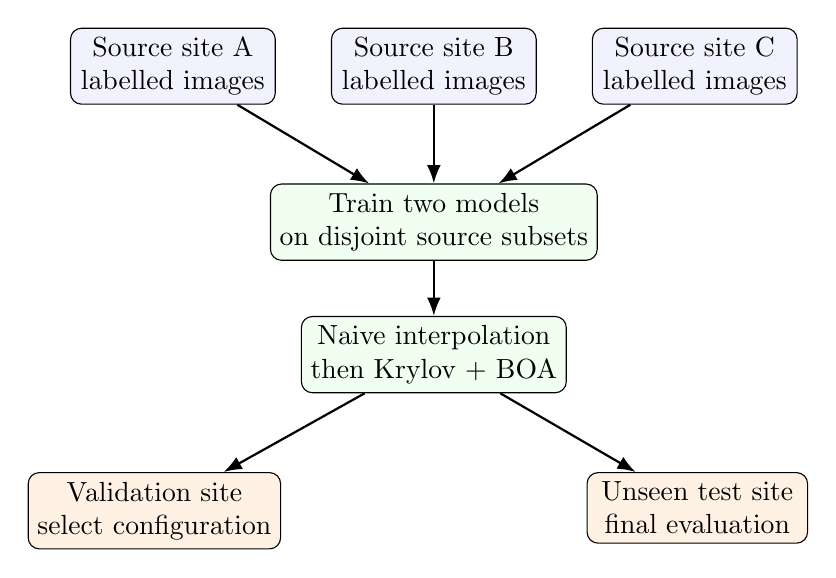
\begin{tikzpicture}[
 node distance=0.7cm and 0.7cm,
 site/.style={draw,rounded corners,align=center,minimum width=2.6cm,minimum height=0.8cm,fill=blue!5},
 proc/.style={draw,rounded corners,align=center,minimum width=3.2cm,minimum height=0.85cm,fill=green!6},
 output/.style={draw,rounded corners,align=center,minimum width=2.8cm,minimum height=0.8cm,fill=orange!10},
 arr/.style={-Latex,thick}
]
\node[site] (s1) {Source site A\\labelled images};
\node[site,right=of s1] (s2) {Source site B\\labelled images};
\node[site,right=of s2] (s3) {Source site C\\labelled images};
\node[proc,below=1.0cm of s2] (train) {Train two models\\on disjoint source subsets};
\node[proc,below=of train] (kry) {Naive interpolation\\then Krylov + BOA};
\node[output,below left=1.0cm and 0.25cm of kry] (val) {Validation site\\select configuration};
\node[output,below right=1.0cm and 0.25cm of kry] (test) {Unseen test site\\final evaluation};
\draw[arr] (s1) -- (train);
\draw[arr] (s2) -- (train);
\draw[arr] (s3) -- (train);
\draw[arr] (train) -- (kry);
\draw[arr] (kry) -- (val);
\draw[arr] (kry) -- (test);
\end{tikzpicture}
\caption{Illustrative wildlife camera-trap deployment scenario. The validation and test locations are kept separate to avoid selecting the final model on the test environment.}
\label{fig:application}
\end{figure}

This scenario is an application proposal, not a field deployment validated by the reported experiments. The TerraIncognita benchmark provides a relevant real-world photographic domain-shift test in the supplied work, but the manuscript does not report a deployed camera system or operational wildlife-monitoring study. A credible application evaluation would require location-wise splits, per-species metrics, confidence intervals, tests for class imbalance, and examination of failure cases in low-light or partially occluded images.

\section{Broader Impact}

A post-training refinement method for domain generalization could be useful in applications where a model must operate across changing visual environments. Examples include environmental monitoring, agricultural inspection, industrial quality control, and visual systems that process images from multiple cameras. In these settings, unexpected changes in acquisition conditions can reduce reliability even when the underlying task remains unchanged. A method that improves a model without requiring a complete retraining cycle may reduce the engineering effort needed to update a deployed system.

The broader value of KryLMC should nevertheless be assessed cautiously. The supplied experiments do not demonstrate performance in a safety-critical deployment, and the current evaluation protocol does not provide a fully controlled unseen-domain test for the main results. It would be inappropriate to infer that the method makes a classifier reliable under arbitrary distribution shifts. Performance may vary with the architecture, the pretraining source, the degree of compatibility between the two trained models, and the geometry of the local loss surface.

There are also computational considerations. The additional basis construction and BOA trajectory evaluations consume processing time and memory. The measured ablation costs show that basis construction grows with the Krylov dimension. For resource-constrained deployment environments, the refinement may therefore be most attractive when it can be performed offline and when the resulting model offers a measurable improvement over the existing baseline.

A responsible deployment should retain a separate evaluation set from each relevant target environment, inspect class-wise errors, and monitor performance after release. The use of image datasets also raises privacy and governance questions where images contain people, private property, or sensitive locations. Dataset provenance, consent, access controls, and retention rules should be addressed by the application owner. The method itself does not solve these data-governance concerns.

\section{Github Link of the Source Code}

\textbf{Code Repository:} 
\href{https://github.com/Anugrah-code/BTP-}{\textbf{https://github.com/Anugrah-code/BTP-}}

% \textbf{Repository:} The public repository URL was not included in the supplied materials. Insert the verified URL here before submission.

% For a reproducible release, the repository should include the training script, interpolation and BOA implementation, model configuration files, environment requirements, random-seed settings, dataset preparation instructions, and commands for reproducing each table. Dataset files and pretrained checkpoints should be referenced through their official sources rather than uploaded when their licences do not permit redistribution. Each result should be accompanied by a configuration file and a log containing the seed, data split, model checkpoint, and evaluation protocol.

\section{Plagiarism and LLM Usage Statement}

The report text has been newly drafted and reorganized from the supplied project manuscript and template. Prior research methods, datasets, and findings are identified through citations; their technical ideas are not presented as original contributions of this project. No percentage of textual similarity is claimed because no institutional plagiarism checker has been run. An LLM-based assistant (ChatGPT) was used to support outlining, language refinement, and LaTeX drafting. It did not conduct the experiments, generate the reported measurements, or independently validate the cited results. The authors are responsible for checking every technical statement, reference, numerical result, and final submission against the original papers, code, and experiment logs.

\begin{thebibliography}{99}

\bibitem{quinonero2009dataset}
J. Qui\~nonero-Candela, M. Sugiyama, A. Schwaighofer, and N. D. Lawrence, eds.,
\emph{Dataset Shift in Machine Learning}. MIT Press, 2009.

\bibitem{bendavid2010theory}
S. Ben-David, J. Blitzer, K. Crammer, A. Kulesza, F. Pereira, and J. W. Vaughan,
``A theory of learning from different domains,'' \emph{Machine Learning}, vol. 79, pp. 151--175, 2010.

\bibitem{blanchard2011generalizing}
G. Blanchard, G. Lee, and C. Scott,
``Generalizing from several related classification tasks to a new unlabeled sample,''
in \emph{Advances in Neural Information Processing Systems}, 2011.

\bibitem{muandet2013domain}
K. Muandet, D. Balduzzi, and B. Sch\"olkopf,
``Domain generalization via invariant feature representation,''
in \emph{Proceedings of the 30th International Conference on Machine Learning}, 2013.

\bibitem{gulrajani2021search}
I. Gulrajani and D. Lopez-Paz,
``In search of lost domain generalization,''
in \emph{International Conference on Learning Representations}, 2021.

\bibitem{ganin2016dann}
Y. Ganin et al.,
``Domain-adversarial training of neural networks,''
\emph{Journal of Machine Learning Research}, vol. 17, no. 59, pp. 1--35, 2016.

\bibitem{li2018conditional}
Y. Li, M. Gong, X. Tian, T. Liu, and D. Tao,
``Domain generalization via conditional invariant representations,''
in \emph{Proceedings of the AAAI Conference on Artificial Intelligence}, 2018.

\bibitem{arjovsky2019irm}
M. Arjovsky, L. Bottou, I. Gulrajani, and D. Lopez-Paz,
``Invariant risk minimization,'' arXiv:1907.02893, 2019.

\bibitem{finn2017maml}
C. Finn, P. Abbeel, and S. Levine,
``Model-agnostic meta-learning for fast adaptation of deep networks,''
in \emph{Proceedings of the 34th International Conference on Machine Learning}, 2017.

\bibitem{balaji2018metareg}
Y. Balaji, S. Sankaranarayanan, and R. Chellappa,
``MetaReg: Towards domain generalization using meta-regularization,''
in \emph{Advances in Neural Information Processing Systems}, vol. 31, 2018.

\bibitem{li2018learninggeneralize}
D. Li, Y. Yang, Y.-Z. Song, and T. M. Hospedales,
``Learning to generalize: Meta-learning for domain generalization,''
in \emph{Proceedings of the AAAI Conference on Artificial Intelligence}, 2018.

\bibitem{zhou2021mixstyle}
K. Zhou, Y. Yang, Y. Qiao, and T. Xiang,
``Domain generalization with MixStyle,''
in \emph{International Conference on Learning Representations}, 2021.

\bibitem{xu2021randomconv}
Z. Xu, D. Liu, J. Yang, C. Raffel, and M. Niethammer,
``Robust and generalizable visual representation learning via random convolutions,''
in \emph{International Conference on Learning Representations}, 2021.

\bibitem{xu2021fourier}
Q. Xu, R. Zhang, Y. Zhang, Y. Wang, and Q. Tian,
``A Fourier-based framework for domain generalization,''
in \emph{Proceedings of the IEEE/CVF Conference on Computer Vision and Pattern Recognition}, 2021, pp. 14383--14392.

\bibitem{volpi2018adversarial}
R. Volpi, H. Namkoong, O. Sener, J. C. Duchi, V. Murino, and S. Savarese,
``Generalizing to unseen domains via adversarial data augmentation,''
in \emph{Advances in Neural Information Processing Systems}, vol. 31, 2018.

\bibitem{zhou2020deep}
K. Zhou, Y. Yang, T. Hospedales, and T. Xiang,
``Deep domain-adversarial image generation for domain generalisation,''
in \emph{Proceedings of the AAAI Conference on Artificial Intelligence}, 2020.

\bibitem{hochreiter1997flat}
S. Hochreiter and J. Schmidhuber,
``Flat minima,'' \emph{Neural Computation}, vol. 9, no. 1, pp. 1--42, 1997.

\bibitem{keskar2017large}
N. S. Keskar, D. Mudigere, J. Nocedal, M. Smelyanskiy, and P. T. P. Tang,
``On large-batch training for deep learning: Generalization gap and sharp minima,''
in \emph{International Conference on Learning Representations}, 2017.

\bibitem{dinh2017sharp}
L. Dinh, R. Pascanu, S. Bengio, and Y. Bengio,
``Sharp minima can generalize for deep nets,''
in \emph{Proceedings of the 34th International Conference on Machine Learning}, 2017.

\bibitem{jiang2020fantastic}
Y. Jiang et al.,
``Fantastic generalization measures and where to find them,''
in \emph{International Conference on Learning Representations}, 2020.

\bibitem{foret2021sharpness}
P. Foret, A. Kleiner, H. Mobahi, and B. Neyshabur,
``Sharpness-aware minimization for efficiently improving generalization,''
in \emph{International Conference on Learning Representations}, 2021.

\bibitem{cha2021swad}
J. Cha et al.,
``SWAD: Domain generalization by seeking flat minima,''
in \emph{Advances in Neural Information Processing Systems}, vol. 34, 2021, pp. 22405--22418.

\bibitem{wang2023sagm}
P. Wang, Z. Zhang, Z. Lei, and L. Zhang,
``Sharpness-aware gradient matching for domain generalization,''
in \emph{Proceedings of the IEEE/CVF Conference on Computer Vision and Pattern Recognition}, 2023.

\bibitem{li2025consistent}
A. Li, L. Zhuang, X. Long, M. Yao, and S. Wang,
``Seeking consistent flat minima for better domain generalization via refining loss landscapes,''
in \emph{Proceedings of the IEEE/CVF Conference on Computer Vision and Pattern Recognition}, 2025, pp. 15349--15359.

\bibitem{song2025dgsam}
Y. Song, Y. Hwang, J. Lee, H. Lee, and D.-Y. Lim,
``DGSAM: Domain generalization via individual sharpness-aware minimization,'' 2025.

\bibitem{wen2023sharpness}
K. Wen, Z. Li, and T. Ma,
``Sharpness minimization algorithms do not only minimize sharpness to achieve better generalization,''
in \emph{Advances in Neural Information Processing Systems}, vol. 36, 2023, pp. 1024--1035.

\bibitem{zhang2021flatness}
S. Zhang, I. Reid, G. V. P\'erez, and A. Louis,
``Why flatness does and does not correlate with generalization for deep neural networks,'' 2021.

\bibitem{li2018visualizing}
H. Li, Z. Xu, G. Taylor, C. Studer, and T. Goldstein,
``Visualizing the loss landscape of neural nets,''
in \emph{Advances in Neural Information Processing Systems}, 2018.

\bibitem{garipov2018loss}
T. Garipov, P. Izmailov, D. Podoprikhin, D. P. Vetrov, and A. G. Wilson,
``Loss surfaces, mode connectivity, and fast ensembling of DNNs,''
in \emph{Advances in Neural Information Processing Systems}, vol. 31, 2018.

\bibitem{draxler2018barriers}
F. Draxler, K. Veschgini, M. Salmhofer, and F. Hamprecht,
``Essentially no barriers in neural network energy landscape,''
in \emph{Proceedings of the 35th International Conference on Machine Learning}, 2018.

\bibitem{frankle2020linear}
J. Frankle, G. K. Dziugaite, D. M. Roy, and M. Carbin,
``Linear mode connectivity and the lottery ticket hypothesis,''
in \emph{Proceedings of the 37th International Conference on Machine Learning}, 2020.

\bibitem{izmailov2018swa}
P. Izmailov, D. Podoprikhin, T. Garipov, D. Vetrov, and A. G. Wilson,
``Averaging weights leads to wider optima and better generalization,''
in \emph{Uncertainty in Artificial Intelligence}, 2018.

\bibitem{wortsman2022soups}
M. Wortsman et al.,
``Model soups: Averaging weights of multiple fine-tuned models improves accuracy without increasing inference time,''
in \emph{Proceedings of the 39th International Conference on Machine Learning}, 2022.

\bibitem{ainsworth2023git}
S. K. Ainsworth, J. Hayase, and S. Srinivasa,
``Git re-basin: Merging models modulo permutation symmetries,''
in \emph{International Conference on Learning Representations}, 2023.

\bibitem{entezari2022permutation}
R. Entezari, H. Sedghi, O. Saukh, and B. Neyshabur,
``The role of permutation invariance in linear mode connectivity of neural networks,''
in \emph{International Conference on Learning Representations}, 2022.

\bibitem{ilharco2023taskarithmetic}
G. Ilharco et al.,
``Editing models with task arithmetic,''
in \emph{International Conference on Learning Representations}, 2023.

\bibitem{saad2003iterative}
Y. Saad, \emph{Iterative Methods for Sparse Linear Systems}, 2nd ed. SIAM, 2003.

\bibitem{liesen2013krylov}
J. Liesen and Z. Strako\v{s}, \emph{Krylov Subspace Methods: Principles and Analysis}. Oxford University Press, 2013.

\bibitem{vinyals2012krylov}
O. Vinyals and D. Povey,
``Krylov subspace descent for deep learning,''
in \emph{Proceedings of the 15th International Conference on Artificial Intelligence and Statistics}, 2012, pp. 1261--1268.

\bibitem{pearlmutter1994hessian}
B. A. Pearlmutter,
``Fast exact multiplication by the Hessian,''
\emph{Neural Computation}, vol. 6, no. 1, pp. 147--160, 1994.

\bibitem{martens2010hessianfree}
J. Martens,
``Deep learning via Hessian-free optimization,''
in \emph{Proceedings of the 27th International Conference on Machine Learning}, 2010, pp. 735--742.

\bibitem{li2026krylovboa}
A. Li, L. Zhuang, X. Long, H. Li, and S. Wang,
``Exploring mode connectivity in Krylov subspace for domain generalization,''
in \emph{International Conference on Learning Representations}, 2026. [Online]. Available: \url{https://openreview.net/forum?id=fpH2GYXJwD}

\bibitem{li2017deeper}
D. Li, Y. Yang, Y.-Z. Song, and T. M. Hospedales,
``Deeper, broader and artier domain generalization,''
in \emph{Proceedings of the IEEE International Conference on Computer Vision}, 2017.

\bibitem{fang2013unbiased}
C. Fang, Y. Xu, and D. N. Rockmore,
``Unbiased metric learning: On the utilization of multiple datasets and web images for softening bias,''
in \emph{Proceedings of the IEEE International Conference on Computer Vision}, 2013, pp. 1657--1664.

\bibitem{beery2018recognition}
S. Beery, G. Van Horn, and P. Perona,
``Recognition in terra incognita,''
in \emph{Proceedings of the European Conference on Computer Vision}, 2018, pp. 456--473.

\bibitem{venkateswara2017deep}
H. Venkateswara, J. Eusebio, S. Chakraborty, and S. Panchanathan,
``Deep hashing network for unsupervised domain adaptation,''
in \emph{Proceedings of the IEEE Conference on Computer Vision and Pattern Recognition}, 2017, pp. 5018--5027.

\bibitem{peng2019moment}
X. Peng, Q. Bai, X. Xia, Z. Huang, K. Saenko, and B. Wang,
``Moment matching for multi-source domain adaptation,''
in \emph{Proceedings of the IEEE/CVF International Conference on Computer Vision}, 2019, pp. 1406--1415.

\bibitem{he2016deep}
K. He, X. Zhang, S. Ren, and J. Sun,
``Deep residual learning for image recognition,''
in \emph{Proceedings of the IEEE Conference on Computer Vision and Pattern Recognition}, 2016, pp. 770--778.

\bibitem{dosovitskiy2021image}
A. Dosovitskiy et al.,
``An image is worth 16x16 words: Transformers for image recognition at scale,''
in \emph{International Conference on Learning Representations}, 2021.

\bibitem{gu2023mamba}
A. Gu and T. Dao,
``Mamba: Linear-time sequence modeling with selective state spaces,'' arXiv:2312.00752, 2023.

\bibitem{oquab2024dinov2}
M. Oquab et al.,
``DINOv2: Learning robust visual features without supervision,''
\emph{Transactions on Machine Learning Research}, 2024.

\bibitem{ridnik2021imagenet}
T. Ridnik, E. Ben-Baruch, A. Noy, and L. Zelnik-Manor,
``ImageNet-21K pretraining for the masses,''
in \emph{Advances in Neural Information Processing Systems, Datasets and Benchmarks Track}, 2021.

\bibitem{paszke2019pytorch}
A. Paszke et al.,
``PyTorch: An imperative style, high-performance deep learning library,''
in \emph{Advances in Neural Information Processing Systems}, vol. 32, 2019, pp. 8024--8035.

\bibitem{rw2019timm}
R. Wightman, ``PyTorch image models,'' 2019. [Online]. Available: \url{https://github.com/huggingface/pytorch-image-models}

\bibitem{kingma2015adam}
D. P. Kingma and J. Ba,
``Adam: A method for stochastic optimization,''
in \emph{International Conference on Learning Representations}, 2015.

\bibitem{loshchilov2017sgdr}
I. Loshchilov and F. Hutter,
``SGDR: Stochastic gradient descent with warm restarts,''
in \emph{International Conference on Learning Representations}, 2017.

\bibitem{kiefer1953sequential}
J. Kiefer,
``Sequential minimax search for a maximum,''
\emph{Proceedings of the American Mathematical Society}, vol. 4, no. 3, pp. 502--506, 1953.

\bibitem{noori2025optimization}
H. Noori, R. Besharat, and M. Z. Mehrzad,
``Optimization of one-dimensional functions using the golden section search method,''
\emph{Journal of Natural Science Review}, vol. 3, no. 3, pp. 59--80, 2025.

\end{thebibliography}

\end{document}
